\chapter{Introduction}
\section{Domain} 
\subsection{Overview}
%TODO application types
Wireless Sensor Networks (WSNs) have received large amounts of research the past decades. However this mainly resulted in isolated ad hoc networks. With both the size of WSN's and the amount of networks increasing, the deployment of multiple networks in the same area for different applications made less and less sense. Therefore, recent endeavours have attempted design networks and protocols in order to create a general, ubiquitous internet for automated devices and sensors: the Internet of Things (IoT).

The recent development in IoT has manly focussed on the field of Low Power Wide Area networks (LPWA). These networks serve devices that communicate over large distances with limited computational and communication resources. They therefore entail low data rates, low radio frequencies and raw unprocessed data. These extremely restrictive requirements entail that a regular wireless internet connection does not suffice, as it is not optimized for the extreme resource limitations of LWPA IoT applications.

The scientific progression in the field of IoT has in turn spaked recent commercial interests. Multiple corporations are deveoping and deploying wide area networks for low powered devices. Examples of these networks are Narrow-Band IoT\cite{web:nbiot}, LoRaWAN \cite{web:lora} and Sigfox \cite{web:sigfox}. These networks are deployed and operated by telcom providers and allow instant connectivity by activiating a SIM or network connectivity module. As a consequence large scale LPWA applications are moving from node-hopping and mesh network strategies to operated cell networks \cite{needs source}. Because of the aforementioned reasons the number of connected devices has exploded in the recent years. Estimations vary but a concensus taken from multiple sources predict about 15-30 billion connected devices in 2020. This would imply that by 2020 the number of connected IoT devices will have surpassed the number of consumer electronic devices (e.g. PC's, laptops and phones) \cite{ericson}. 

Both the explosion of devices and entailing explosion of data, and the shift to shared operated cell networks implies a great stress on monitoring sensor applications. While relatively small sized applications on proprietary networks allow for a best-effort approach, the convolution of many large applications on a shared network requires knowledge of the state of the application. The term coined for this is Quality of Service. QoS parameters such as application throughput, service availability and delivery guarantee allow the description of the state of a system or application.
%TODO shortly define scope, stakeholders en business value

\subsection{Challenges of monitoring QoS in IoTs and WSNs}
Though the concept of QoS is well understood, the exist challenges in measuring and determining QoS in WSNs. 
\subsubsection{Technical limitations}
The first challenge of LPWA applications is the aforementioned extreme resource constraints. As a LPWA device is required to perform for a certain amount of time (typically at least 10 years \cite{???}) on a finite, bounded battery energy supply, there are no resources to spare for expensive auxiliary processes. Therefore, devices usually send low-level auxiliary data, instead of intelligently derived values. The burden of calculating high level information is therefore deferred to be computed in-network (edge) or in the back-end.

Additionally, evolution of sensor device software is far more restrictive then evolution of server software. Firstly because of the long life-time of devices, it can occur that services based on modern day requirements need to be performed on decade old technology. Secondly, most LWPA networking protocols do not require devices to retain a constant connection, in order to save energy\cite{tmobile, vodafone, iets met nbiot specs}. Instead the devices connect periodically or when an event/interrupt occurs. This entails that devices cannot be updated \emph{en masse}, but individually when a device wakes up. As this requires additional resends of the updated code it consumes more connectivity resources in the network. For this reason LPWA sensor applications often employ a \emph{"dumb sensor, smart back-end"} philosophy. Again deferring the computations to the network or the back-end.

The problem however with deferring the computations further to the back-end is that more and more computations have to be performed centralized. This requires the back-end to be extremely scalable as more jobs need to be performed as more devices are added to the application.

\subsubsection{Why IoT QoS is different}
Aside from the low-level information sent by the large amout of devices, QoS in WSNs is distinctly different from classical client-server based QoS. Often QoS in a server-based applicaiton can be measured at the server. QoS may need aggegation when the service is run on a cloud environment, but even then the number of data sources is relatively limited. Large WSN applications require data aggegation by default. As the level of service provided by the application can only be assertained by calculation based on temporal auxiliary data collected from the devices. This concept is known as Collective QoS \cite{collective_qos} and comprises parameters such as collective bandwidth, average throughput and the number of devices that require replacement. As this information eventually requires accumulation on a single machine in order to determine singular values, aggregation of expansive amounts of auxiliary sensor data must be aggregated intelligently as to not form a congestion point or single point of failure.

Alongside of collective QoS we still require device level information. If a device is not performing according to expectations of the predetermined strategy, it is required that this is notified. This introduces a second distinction to classical QoS: multi-level monitoring and reporting. Usually we are only interested in the QoS provided by the sever(s) running our application. However in a wireless sensor environment we require monitoring parameters on different levels. Examples of these monitoring levels are single sensor, the application as a whole or analysis per IoT cell tower or geographic area. This requirement entails data points of different levels of enrichment, calculated from the same raw sensor data.

The final distinction in IoT monitoring is the dynamic nature of WSN applications. An IoT monitoring application needs to be prepared for devices added to the network and dropping out of the application is prone to change of scale and devices are prone to failure and replacement. As a collective QoS parameter is based on a selection of devices, the monitoring application must support adding and remove devices from the equation.

\subsubsection{Movement to operated cell network}
A final challenge in contemporary QoS monitoring of LPWA applications is the earlier recognised increasing trend of commercial telecom operated cell networks. Though is makes IoT connectivity more efficient because many applications can be served by a single network infrastructure, it does pose some difficulties to QoS. Firstly, Many applications will be competing for a shared scarce amount of network resources. When other applications consume a large portion of the resources, due to poor rationing or event-bursts, your application suffers and cannot provide expected QoS.

Secondly, by out-sourcing the network infrastructure control over the network is lost. Though beneficiary to the required effort, some important capabilities are conceded. For example the network can no longer be easily altered in order to suit the needs of the application. Additionally, auxiliary data can not be extracted from the network and edge computing is not an option, deferring the burden of aggregating QoS data entirely on back-end.

Finally, the telecom operator will require adherence to a Service Level Agreement (SLA). Though this ensures a certain service provided to an application and prevents other applications of consuming extraneous resources, it also requires close monitoring of applications. A breach of the SLA may entail fines or a breach of contract, strict adherence to the SLA parameters and proactive intervention if the limits of the SLA are threatened to be exceeded. \cite{zoek refs in rtopics}

\section{State of affairs}
Several platforms exist that are capable monitoring and controlling IoT applications to some degree \cite{refs_to_platoforms}. However all are lacking in some of the important considerations. These platforms are either not conceived with a focus on LPWA's severe resource constraints, a primary focus on resource and QoS monitoring or the extreme scale of contemporary WSN applications \cite{platform surveys}.

These deficiencies make the existing monitoring platforms insufficient solutions for monitoring and controlling large scale LPWA IoT applications. This implies that the technologies are either inapplicable or require a composition of these technologies. This complication of the technology stack would be acceptable for a key function of an application, but not for an auxiliary monitoring processes. As to not complicate a software product which does not enjoy the main focus of development efforts it would be beneficiary to have a single platform which enables it's development.

\section{Goal}
The goal of this study is to research and develop a single platform capable of measuring and monitoring. This platform will enable development support applications that process auxiliary IoT data. This data is raw and low-level, but is enriched by the platform by associating streaming data with data obtained from relevant data sources and aggregating streaming data to infer higher-level information. this information can be exported for reporting and visualization purposes, can alter the state of a system (single sensor, group of sensors, entire application, etc.) and can cause alerts to be dispatched for immediate intervention.

\subsection{Research questions}
To accomplish the goal set out for this study the following question require answering.
\begin{enumerate}[leftmargin=24pt, label=\small RQ\arabic*]
\nospace
\item What are the key data transformations and operations that are performed on (auxiliary) data streams generated by WSNs?
\item How to design a platform that facilitates the identified WSN data streams, transactions and operations?
\item What is the appropriate level of abstraction for a WSN monitoring platform, such that
\begin{itemize}
\nospace
\item the platform is applicable to monitoring a large domain of WSNs, and
\item allows for the highest ease-of-implementation?
\end{itemize}
\item What are the challenges regarding scalability in a WSN data stream processing platform?
\item How can these challenges be overcome?
\item What are the key concepts regarding modelling and calculation of QoS parameters?
\item How can we model the state of a system with variable behaviour?
\item How can we determine the optimal system behaviour in accordance with its state?
\end{enumerate}

From the listed research questions we find a focus that is twofold. The first point of focus is the composition and development of an abstract, scalable streaming platform for IoT data enrichment. The associative questions are RQ1-5. It concerns the appropriate abstraction of a platform combatting the challenges in iteratively refining low-level sensor data to high-level information with business value and scalability due to the vast amount of data generated by the WSN.  The second focal point concerns the representation and processing of information depicting the state of a system. This entails capturing some data points produced by sensor devices or intermediary processes, calculating the derived parameters from those measurements and producing a decision in accordance with the model's values and set rules.

\subsection{Scope and stakeholders}
%scope
%iot en wsn
%abstract
%	monitor
%	iput: high volume low information measurements
%		related, but not neccesarily same object
%	require: high level information for reporting or (automated) decision making
%stakeholders (onion model)

%TODO Waarom?
Another approach to scope our efforts is by identifying the stakeholders for our platform. We will perform this by analogy of the Onion Stakeholder Model as proposed by [ref]\cite{onion}. This model divides stakeholders in consecutive layers, ordered by the degree of interaction and benefits received from the product. For the stakeholder division we will consider the product to be both the platform to be developed and potential future implementations of the platform. Intuitively, this project definition would result in a two level product in the model, with the platform as core and the group of all instantiations al the first layer around it. However since this analysis focusses on human stakeholders, we will treat it as a single instance in our application of the model. A visual representation of the application of the onion model is given in Figure \ref{fig:onion}.

The first layer of the model directly encasing the product is \textbf{Our System}. It encompasses the designed and developed product (i.e. the platform and its instances) and the human parties that directly interface with the product. The first group of these stakeholders is the \emph{Employee Developing and Maintaining} implementations of the platform. They interact directly with scaffolding and frameworks provided by the core platform. Some explanations of the onion model place developers in the outer layer of the model (the wider environment), since after development they no longer interface with the product unless they remain involved in a maintenance capacity. However, since developers of a platform instantiation interact with the scaffolding and frameworks directly provided by the core platform, we emphasize their importance by placing them in the system layer of the model. The second role in the system layer is the \emph{Normal Operator}. These operators receive information from the product directly and interact with subsequent systems and operational support employees to effect change. For our product this entails changes to the application under investigation or reports regarding the long term performance of the application to be forwarded to managers and employees higher up in the organization.

The second layer of the model is the \textbf{Containing System}. It contains stakeholders that are heavily invested in the performance and benefits of the product, but do not interact with it directly on a regular basis. We have identified two of these stakeholder roles. The first is the \emph{Support and Maintenance Operator} of the application observed by the platform. If we were to analyse the stakeholders of the application under investigation, these operators would be placed in the first layer of the model. However since they do not (necessarily) directly interface with our support platform, they are placed in the second layer of the model for our product. They are however heavily invested in the performance and results of the platform, since identified problems and deficiencies can direct their efforts toward maintaining and improving their own application. The second role in this layer is the \emph{Sales Person} of the application under investigation. Again this regards a sales person of the application under investigation, not our support platform. The task of a sales person is to convince potential clients to employ a developed product. Performance guarantees are an important part of a sales pitch held by this type of stakeholder. Therefore employees of sales departments benefit hugely from known, concrete and stable QoS metrics.

The third layer of the model is the \textbf{Wider Environment}. This final layer contains stakeholders that do not sentiently interface with the product and are not heavily or conciently interested in its execution or performance, but are affected by it to some degree. The first stakeholder role in this category is the \emph{Financial Benefactor}. This entity is not heavily invested in the development and dayly routine of the system, but does benefit financially from it. This role applies to investors, companies and other business units that are not concerned with the technical upkeep of the product, but do benefit from the gained revenue or cost-efficient measures provided by the product. Closely related with this is the \emph{Political Benefactor}. This benefactor does not directly reap monetary benefit from the solution, but does gain political benefit from it. This can apply to both stakeholders in public office or private business by improving their position in their respective markets. The final stakeholder is the \emph{General Public}. Members of the public do not interface with our platform in any capacity, but can benefit heavily from it. For example, many WSN and IoT applications are deployed in smart city management and industry4.0\cite{voorbeelden}. Though deployment of dependable IoT technologies in these fields require initial investments, in the long term these technologies can improve efficiency, reducing costs and prizes. Therefore, guaranteed uptime and low resource usage can benefit the consumer, without them realizing it. Though the benefit to singular consumers are relatively small, due to the huge size of the public at large this amounts to a incredible benefit.

\begin{figure}
\centering
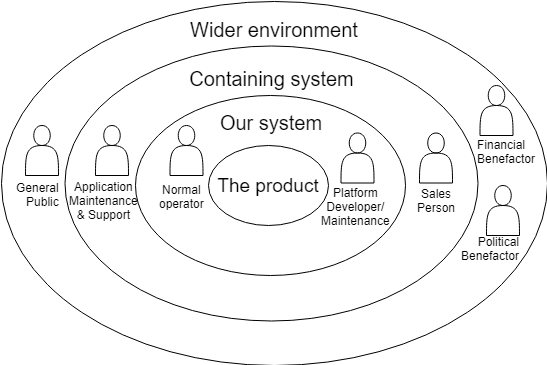
\includegraphics[width=.7\textwidth]{resources/img/onion.png}
\caption{Visual depiction of application of onion stakeholder model}
\label{fig:onion}
\end{figure}

\section{Approach}
With the goal and purpose of this research clear the aimed upon methodology requires clarification. As the above section mentioned the research questions can be divided into two categories: The platform and modelling resource distribution. Our approach is therefore to research these individually before integrating these efforts into one resulting software development platform. 

Each point of focus will be devised, designed and developed according to the following schedule. We will first explore the problem domain of the to be designed solution/model. This will be performed with a commonality/variability analysis (section \ref{sec:back:cv_analysis}). This analysis allows us to conceptualize the problem domain which will result in a list of requirements for the solution to adhere to. With the requirements defined the state of the art of the problem domain will be explored to identify viable technologies and their deficiencies, before selecting the best applicable technologies. With these technologies identified we will adapt, design and develop the intended artifact. For design and development we will adopt the iterative development approach of Design Science Methodology\cite{dsm} (section \ref{sec:back:dsm}). Ultimately, the devised solution will be evaluated and discussed by paralleling them to the set requirements and some additional concepts and criteria. 

Once the two compounds have been integrated into a single solution, the challenges it claims to combat will need verifying. In order to perform initial validation of the developed solution it will be applied to a real-world commercial car park WSN application developed and maintained by the Dutch company Nedap N.V.
%TODO diclaimer partial validation

\section{Organisation of thesis}
%TODO finally do